\documentclass[a4paper,french,bookmarks]{article}
\usepackage{./Structure/4PE18TEXTB}

\begin{document}
\stylize{Sciences de L'ingénieur}{Devoir Maison 1 : Position d'un sous-marin autonome}

\begin{enumerate}
    \item Déterminer l'unité de gain $A$
    
    \boxans {
        On a $f(t)=Au(t)$ donc $A = \dfrac{u(t)}{f(t)}$.
        
        On trouve alors comme unité pour le gain $A$ le \boxsol{\textit{Newton par Volt} ($N\cdot V^{-1}$)}
    }
    
    \item Déterminer les fonctions de transfert $H_1$, $H_2$ et $H_3$
    
    \boxans{
        Premièrement, on a $F(p) = H_1(p)U(p)$, donc $H_1(p)=\dfrac{F(p)}{U(p)}$. Or d'après $(Eq1)$, on a $f(t)=Au(t)$.
        
        Donc $H_1(p)=\dfrac{\lap{f(t)}}{U(t)}=\dfrac{AU(p)}{U(p)}$ donc \boxsol{$H_1(p)=A$}. 
        
        Deuxièmement, on a $V(p)=H_2(p)F(p)$, donc $H_2(p)=\dfrac{V(p)}{F(p)}$. D'après $(Eq2)$, on a $Kf(t)=v(t)+\tau\difft v(t)$.
        
        Donc $\lap{Kf(t)}=V(p)+\tau pV(p)=V(p)(1+\tau p)$, soit $V(p)=\dfrac{KF(p)}{1+\tau p}$. Donc \boxsol{$H_2(p)=\dfrac{K}{1+\tau p}$}.
        
        Troisièmement, on a $X(p)=H_3(p)V(p)$, donc $H_3(p)=X(p)/V(p)$. Par définition, $v(t)=\difft x(t)$.
        
        Donc $\lap{v(t)} = pX(p)$ soit $X(p)=\dfrac{V(p)}{p}$. Donc \boxsol{$H_3(p)=\dfrac{1}{p}$}.

    }
    
    \item Déterminer l'expression de la fonction de transfert $G(p)=\dfrac{X(p)}{U(p)}$ de la         chaîne d'action reliant la tension à la position en fonction de la variable $p$ et des        constantes $A$, $k$ et $\tau$. On pose $A = 200 \ S.I$, $K = 5\cdot 10^{-3} \ s\cdot kg^{-1}$ et $\tau = 5,5 \ s$.
    
    \boxans{
        On a $\left\lbrace\begin{array}{ll}
            X(p) &=  H_3(p)V(p)\\
            V(p) &=  H_2(p)F(p)\\
            F(p) &=  H_1(p)U(p)
        \end{array}\right.$ donc $X(p)=H_3(p)H_2(p)H_1(p)U(p)=\dfrac{AK}{p(1+\tau p)}U(p)$.
        
        Avec $G(p)=\dfrac{X(p)}{U(p)}$, on a donc \boxsol{$G(p)=\dfrac{AK}{p(1+\tau p )}=\dfrac{1}{p+5,5p^2}$}
    }
    
    %Le système étant initialement au repos ($u(t) = 0$ et $x(t) = 0$ pour $t < 0$), on établit instantanément à $t = 0$, une tension de commande, d'amplitude constante égale à $1$ \textit{Volt} en continu, à l'entrée du bloc propulseur.
    
    \item Quel est le nom de ce signal de commande ? Représentez le sur un graphique. Donnez l'expression simple de sa transformée de Laplace : $U(p)$.
    
    \boxans{
       La fonction $u(t)$, est appelé \boxsol{échelon unité} (ou fonction de Heaviside). On a \boxsol{$U(p)=\lap{u(t)}=\dfrac{1}{p}$}.
        
        \pgfplotsset{height=7cm, width=13cm}
        \center 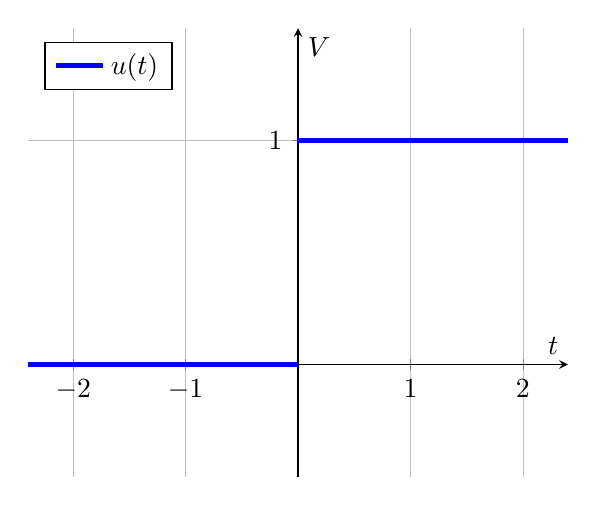
\begin{tikzpicture}
            \begin{axis}[
                axis lines          = center,
                xmin                = -2.4,
                xmax                = 2.4,
                xlabel              = $t$,
                ylabel              = $V$,
                ytick               = {1},
                xtick               = {-2,-1,0,1,2},
                ymin                = -0.5,
                ymax                = 1.5,
                grid                = both,
                grid style          = {line width = .1pt, draw = gray!30},
                major grid style    = {line width=.2pt,draw=gray!50},
                minor tick num      = 0,
                legend pos          = north west,
            ]
            
            \addplot[domain=0:2.4, color=blue, line width=0.6mm] {1};
            \addlegendentry{$u(t)$}
            \addplot[domain=-2.4:0, color=blue, line width=0.6mm] {0};
            
            \end{axis}
        \end{tikzpicture}
    }
    
    \item Déterminer et tracer l'allure de la réponse $x(t)$ à ce signal.
    
    \boxans{
        On a $G(p)=\dfrac{X(p)}{U(p)}$ donc $X(p)=G(p)U(p)$. De plus $G(p)=\dfrac{AK}{p(1+\tau p)}$ et $U(p)=\dfrac{1}{p}$.
        
        Donc $X(p)=\dfrac{AK}{p^2(1+\tau p )}$. On réduit en éléments simples : on pose $(a,b,c) \in \bdR^3$ tels que :
        \[ X(p) = AK\left(\dfrac{a}{p}+\dfrac{b}{p^2}+\dfrac{c}{1+\tau p}\right)=AK\left(\dfrac{ap(1+\tau p)+b(1+\tau p)+cp^2}{p^2(1+\tau p)}\right)=AK\dfrac{1}{p^2(1+\tau p)}\]
        
        Donc $ap(1+\tau p)+b(1+\tau p)+cp^2 = 1$ soit $ap+a\tau p^2 + b + b\tau p + cp^2 = 1$ donc :
        \[ \left\lbrace\begin{array}{lc}
            b &= 1  \\
            a + b\tau &= 0\\
            a\tau + c &= 0
        \end{array}\right. \ \text{donc} \ \left\lbrace\begin{array}{lc}
            b &= 1  \\
            a &= -\tau\\
            c &= \tau^2\\
        \end{array}\right.\]
        Donc $X(p)=AK\left(\dfrac{-\tau}{p}+\dfrac{1}{p^2}+\dfrac{\tau^2}{1+\tau p}\right)=AK\left(-\tau\dfrac{1}{p}+\dfrac{1}{p^2}+\tau\dfrac{1}{p+\frac{1}{\tau}}\right)$.
        
        Par linéarité de la transformée de Laplace, on a donc :
        \[ x(t)=AK\left(-\tau u(t) + tu(t) + \tau e^{-\frac{t}{\tau}}u(t)\right)\]
        Donc finalement, \[ \boxsol{$x(t)=AKu(t)\left(t + \tau\left(e^{-\frac{t}{\tau}}-1\right)\right)$}\]
        
        Pour $t \geq 0$, l'expression se simplifie en $x(t)=t + 5,5\left(e^{\frac{t}{5,5}}-1\right)$
        
        \pgfplotsset{height=9cm, width=13cm}
        \center \begin{tikzpicture}
            \begin{axis}[
                axis lines          = center,
                xmin                = -3.5,
                xmax                = 7.5,
                xlabel              = $t$,
                ylabel              = $m$,
                ytick               = {1,2,3},
                xtick               = {-2,0,2,4,6},
                ymin                = -0.5,
                ymax                = 3.5,
                grid                = both,
                grid style          = {line width = .1pt, draw = gray!30},
                major grid style    = {line width=.2pt,draw=gray!50},
                minor tick num      = 0,
                legend pos          = north west,
            ]
            \addplot[domain=0:7.5, color=blue!50, style=dashed, line width=0.6mm] {1};
            \addlegendentry{{\color{white5}($u(t)$)}}
            \addplot[color=blue, line width=0.5mm]
            coordinates {
                    (0.0, 0.0)
                    (0.1, 0.0009036361484352218)
                    (0.2, 0.0035927430838888497)
                    (0.3, 0.008035151049496314)
                    (0.4, 0.01419926990765269)
                    (0.5, 0.022054078696711277)
                    (0.6, 0.03156911537584495)
                    (0.7, 0.04271446675467683)
                    (0.8, 0.055460758604357396)
                    (0.9, 0.06977914594681256)
                    (1.0, 0.08564130351895916)
                    (1.1, 0.1030194164087267)
                    (1.2, 0.12188617085979936)
                    (1.3, 0.14221474524203104)
                    (1.4, 0.16397880118455177)
                    (1.5, 0.18715247486863507)
                    (1.6, 0.21171036847744173)
                    (1.7, 0.23762754179982482)
                    (1.8, 0.2648795039854075)
                    (1.9, 0.29344220544821686)
                    (2.0, 0.3232920299161921)
                    (2.1, 0.3544057866239445)
                    (2.2, 0.3867607026461799)
                    (2.3, 0.42033441536925675)
                    (2.4, 0.4551049650983887)
                    (2.5, 0.49105078779804456)
                    (2.6, 0.5281507079631482)
                    (2.7, 0.5663839316187276)
                    (2.8, 0.6057300394456817)
                    (2.9, 0.6461689800304171)
                    (3.0, 0.6876810632360977)
                    (3.1, 0.730246953693336)
                    (3.2, 0.7738476644081635)
                    (3.3, 0.8184645504851682)
                    (3.4, 0.8640793029637268)
                    (3.5, 0.910673942765293)
                    (3.6, 0.9582308147497405)
                    (3.7, 1.0067325818787967)
                    (3.8, 1.0561622194846314)
                    (3.9, 1.1065030096417252)
                    (4.0, 1.1577385356401226)
                    (4.1, 1.2098526765582838)
                    (4.2, 1.2628296019337015)
                    (4.3, 1.3166537665295595)
                    (4.4, 1.3713099051956643)
                    (4.5, 1.4267830278219824)
                    (4.6, 1.483058414383101)
                    (4.7, 1.5401216100719664)
                    (4.8, 1.5979584205213118)
                    (4.9, 1.6565549071111758)
                    (5.0, 1.7158973823609722)
                    (5.1, 1.7759724054045765)
                    (5.2, 1.836766777546952)
                    (5.3, 1.8982675379008196)
                    (5.4, 1.9604619591019565)
                    (5.5, 2.0233375431016882)
                    (5.6, 2.0868820170351907)
                    (5.7, 2.151083329164236)
                    (5.8, 2.2159296448930395)
                    (5.9, 2.2814093428558904)
                    (6.0, 2.3475110110752753)
                    (6.1, 2.414223443189223)
                    (6.2, 2.48153563474662)
                    (6.3, 2.549436779569278)
                    (6.4, 2.61791626617955)
                    (6.5, 2.686963674292304)
                    (6.6, 2.756568771370114)
                    (6.7, 2.826721509240509)
                    (6.8, 2.8974120207741696)
                    (6.9, 2.968630616622988)
                    (7.0, 3.0403677820168835)
                    (7.1, 3.1126141736183426)
                    (7.2, 3.1853606164336306)
                    (7.3, 3.2585981007796496)
                    (7.4, 3.3323177793054573)
            };
            \addlegendentry{$x(t)$}
            \addplot[domain=-3.5:0, color=blue!50, style=dashed, line width=0.6mm] {0};
            \addplot[domain=-3.5:0, color=blue, line width=0.5mm] {0};

            \end{axis}
        \end{tikzpicture}
    }
    
    \item Le système est-il stable ?
    
    \boxans{
        On remarque qu'avec un échelon en entrée, $x(t)$ tend vers l'infini.
        
        Donc \boxsol{Le système n'est pas stable.}
    }
    
    \item Quelle valeur doit avoir le gain d'adaptation $K_a$ pour avoir un écart nul si la consigne $X_C$ et la position réelle $X$ sont identiques.
    
    \boxans{
        On cherche $K_a$ tel que $\epsilon(p)=0$.
        
        On a donc $Ka_XC(p)-BX(p)=0$, soit $Ka_XC(p)=BX(p)$.
        
        Or si la consigne $X_C$ et la position réelle $X$ sont identiques, $X(p)=X_C(p)$.
        
        Donc \boxsol{$K_a=B$}.
    }
    
    \item Déterminer la fonction de transfert en boucle fermée entre la consigne $X_C$ et la position réelle $X$.
    
    \boxans{
    On a $X(p) = FTBF(p)X_C(p)$ donc $FTBF(p) = \dfrac{X(p)}{X_C(p)}$. De plus $\left\lbrace\begin{array}{ll}
            \epsilon(p) &= K_a\cdot X_C(p)-BX(p)  \\
            X(p) &= \epsilon(p)C(p)G(p)
        \end{array}\right.$.
    \[ X(p) = \left(K_a\cdot X_C(p)-BX(p)\right)C(p)G(p) \ \text{soit} \ X(p)(1+BC(p)G(p))=K_aX_C(p)C(p)G(p)\]
    Donc $X(p) = X_C(p)\dfrac{K_aC(p)G(p)}{1+BC(p)G(p)}$, donc \boxsol{$FTBF(p)=\dfrac{K_aC(p)G(p)}{1+BC(p)G(p)}$}
    }
    
    \item Déterminer tous critères de performances de la réponse simulée. Le cahier des charges est-il respecté ?
    
    \boxans{
        Pour $t \approx 30 \ s$, on mesure graphiquement $X\approx 13,7 \ m$. Donc $ 5 \% \times 15 = 0,75 < \mod{15 - 13,7}$.
        
        Donc $\exists t > 30 \ s$, $\mod{X_C - X(t)} > 5\% \cdot X_C$, ainsi \boxsol{le critère de rapidité n'est pas respecté}.
        
        On remarque graphiquement que pour les grandes valeurs de $t$, signal de consigne et réponse temporelle sont confondus, donc \boxsol{le critère de précision est respecté}.
        
        Ainsi, puisque le signal converge, \boxsol{le critère de stabilité est respecté}.
        
        Enfin, on observe graphiquement que \boxsol{le critère de dépassement n'est pas respecté}. 
    }
    
    \item Mettre la fonction de transfert trouvée à la question $8$ sous forme canonique et exprimer les constantes caractéristiques en fonction de $K_c$.
    
    \boxans{
        \[
            FTBF(p) = \dfrac{K_aC(p)G(p)}{1+BC(p)G(p)}
            = \dfrac{K_aK_c\frac{1}{p+5,5p^2}}{1+BK_c\frac{1}{p+5,5p^2}}
            = \dfrac{K_aK_c}{p+5,5p^2+BK_c}
        = \dfrac{\frac{K_a}{B}}{\frac{1}{BK_c}p+\frac{5,5}{BK_c}p^2+1}
        \]
        On prend $K_a = B = 1 \ V \cdot m^{-1}$. On pose $(\omega_0, \eta, K) \in \bdR_+^3$ tels que \boxsol{$FTBF(p) =\dfrac{1}{1+\frac{2\xi}{\omega_0}p+\frac{K}{{\omega_0}^2}p^2}$}.
        
        On a donc $\displaystyle \left\lbrace\begin{array}{ll}
            \dfrac{2\xi}{\omega_0} &= \dfrac{1}{K_c}  \\
            K &= 1\\
            \dfrac{1}{{\omega_0}^2} &= \dfrac{5,5}{K_c}
        \end{array}\right.$ donc \boxsol{$\displaystyle \left\lbrace\begin{array}{ll}
            \xi &= \dfrac{1}{2\sqrt{5,5K_c}}\\
            K &= 1\\
            \omega_0 &= \sqrt{\dfrac{K_c}{5,5}}
        \end{array}\right.$}
    }
    
    \item Déterminer la valeur de $K_C$ pour que le système réponde aux exigences du cahier des charges. Déterminer alors le temps de réponse à 5\%.
    
    \boxans{
        Comme $K = 1$, l'écart statique est nul, donc le critère de précision est respecté.
        On a pris $(\omega_0, \eta) \in \bdR_+^2$ donc $1$, $\dfrac{2\xi}{\omega_0}$ et $\frac{1}{{\omega_0}^2}$ sont de même signes, donc le système est stable.
        
        On cherche à ne pas avoir de dépassement, donc $\xi \geq 1$. Or d'après l'abaque du temps de réponse réduit, la valeur de $t_{r5\%}{\omega_0}$ (en fonction de $\xi$) est croissante sur $[1; +\infty[$.
        Il est donc logique de calculer la valeur optimale de $K_c$ en prenant $\xi = 1$.
        
        On a donc $\dfrac{1}{2\sqrt{5,5K_c}} = 1$, soit $2\sqrt{5,5K_c}=1$ soit $5,5K_c = \dfrac{1}{4}$ donc finalement \boxsol{$K_c = \dfrac{1}{22}$}.
        
        On calcule ensuite $w_0 = \sqrt{\dfrac{K_c}{5,5}} = \dfrac{1}{11}$. Or d'après l'abaque, pour $\xi = 1$, on a $t_{r5\%}{\omega_0}(\xi) \approx 5$ soit $t_{r5\%} \approx \dfrac{5}{\omega_0}$.
        Finalement, on a donc \boxsol{$t_{r5\%} \approx 55\ s$}. 
        
        On remarque que même avec une valeur optimale de $\xi$, on a toujours $t_{r5\%} > 30 \ s$. 
        
        Ainsi, \boxsol{le cahier des charges ne peut être entièrement respecté}.\newline\newline
        
        \textbf{N.B.} Il faudrait donc soit accepter un certain dépassement, soit accepter un temps plus long. La non collision paraissant plus importante, il faudrait donc plutôt sacrifier le critère de rapidité.
    }
    
\end{enumerate}
\end{document}